\documentclass[6pt,letterpaper]{article}
\usepackage[margin=0.25in, top=0.3in, bottom=0.25in]{geometry}
\usepackage{amsmath,amssymb}
\usepackage{multicol}
\usepackage{xcolor}
\usepackage{mdframed}
\usepackage{microtype}
\usepackage{fancyhdr}
\usepackage{booktabs}
\usepackage{colortbl}
\usepackage{array}
\usepackage{graphicx}

% ── Colors ──
\definecolor{purple}{HTML}{534AB7}\definecolor{purplebg}{HTML}{EEEDFE}
\definecolor{teal}{HTML}{0F6E56}\definecolor{tealbg}{HTML}{E1F5EE}
\definecolor{coral}{HTML}{993C1D}\definecolor{coralbg}{HTML}{FAECE7}
\definecolor{amber}{HTML}{854F0B}\definecolor{amberbg}{HTML}{FAEEDA}
\definecolor{green}{HTML}{3B6D11}\definecolor{greenbg}{HTML}{EAF3DE}
\definecolor{blue}{HTML}{0C447C}\definecolor{bluebg}{HTML}{E6F1FB}
\definecolor{gray}{HTML}{444441}\definecolor{graybg}{HTML}{F1EFE8}
\definecolor{pink}{HTML}{72243E}\definecolor{pinkbg}{HTML}{FBEAF0}
\definecolor{rowB}{HTML}{F2F2EF}

\newmdenv[linewidth=0.4pt,innerleftmargin=3pt,innerrightmargin=3pt,
  innertopmargin=2pt,innerbottommargin=2pt,skipabove=1pt,skipbelow=1pt]{ebox}

\newcommand{\shead}[3]{%
  \noindent\colorbox{#1}{\parbox{\dimexpr\linewidth-2\fboxsep\relax}%
  {\color{#2}\bfseries\fontsize{6}{7}\selectfont #3}}\vspace{0.5pt}}

% label + when-to-use on same line
\newcommand{\eq}[2]{\noindent{\color{gray}\bfseries\fontsize{5.8}{6}\selectfont#1}\enspace{\color{teal}\fontsize{5.5}{6}\selectfont\textit{#2}}}

\setlength{\parindent}{0pt}\setlength{\parskip}{0pt}
\setlength{\columnsep}{5pt}\setlength{\multicolsep}{1pt}

\pagestyle{fancy}\fancyhf{}
\renewcommand{\headrulewidth}{0.3pt}
\fancyhead[L]{\fontsize{6.5}{7}\selectfont\textbf{ECE332 --- Exam 1 Cheat Sheet (HW1 + HW2)}}
\fancyhead[R]{\fontsize{6.5}{7}\selectfont Bao Nguyen}

% images live in Midterm1/img/
\graphicspath{{../img/}}

\begin{document}

%%=============================================================
%% PAGE 1 — HW1 CHEAT SHEET (verbatim)
%%=============================================================
\fontsize{6}{7.5}\selectfont
\setlength{\abovedisplayskip}{1pt}\setlength{\belowdisplayskip}{1.5pt}
\setlength{\abovedisplayshortskip}{0pt}\setlength{\belowdisplayshortskip}{0pt}
\begin{multicols}{3}

%──────────────────────────────────────
\shead{purplebg}{purple}{EMF \& FARADAY'S LAW}
\begin{ebox}
\eq{Transformer EMF}{stationary loop, $B$ changes}
\[V_\text{emf} = -\int_S \frac{\partial \mathbf{B}}{\partial t} \cdot d\mathbf{s}\]

\eq{Motional EMF}{loop moves, $B$ static}
\[V_\text{emf} = \oint (\mathbf{v} \times \mathbf{B}) \cdot d\mathbf{l}\]

\eq{General (flux form)}{always works}
\[V_\text{emf} = -\frac{d\Phi}{dt} \qquad \Phi = \int_S \mathbf{B} \cdot d\mathbf{s}\]

\eq{$N$-turn coil}{transformer, $N$ turns}
\[V_\text{emf} = -N\frac{d\Phi}{dt} = -\frac{d\lambda}{dt} \quad \lambda=N\Phi\]

\eq{Uniform $B$ shortcut}{$B$ same everywhere on loop}
\[V_\text{emf} = -\frac{\partial B}{\partial t} \cdot A\]

\eq{Long wire + rect loop}{wire near loop, $r$: $a\to b$, height $c$}
\[V_\text{emf} = -\int_0^c\!\int_a^b \frac{\partial \mathbf{B}}{\partial t} \cdot d\mathbf{s} = -\int_0^c\!\int_a^b \frac{\partial}{\partial t}\!\left(\frac{\mu_0 I}{2\pi r}\right)dr\,dz\]
\end{ebox}

\vspace{2pt}
\shead{purplebg}{purple}{MAXWELL'S EQUATIONS}
\begin{ebox}
{\centering\makebox[0.98\linewidth][c]{{\setlength{\tabcolsep}{2pt}\begin{tabular}{@{}p{0.28\linewidth}p{0.66\linewidth}@{}}
\toprule
Name & Differential form\\
\midrule
\rowcolor{rowB}Faraday & $\nabla\!\times\!\mathbf{E}=-\partial\mathbf{B}/\partial t$\\
Ampère & $\nabla\!\times\!\mathbf{H}=\mathbf{J}+\partial\mathbf{D}/\partial t$\\
\rowcolor{rowB}Gauss\,(E) & $\nabla\!\cdot\!\mathbf{D}=\rho_v$\\
Gauss\,(B) & $\nabla\!\cdot\!\mathbf{B}=0$\\
\bottomrule
\end{tabular}}}\par}
\textit{$\mathbf{D}=\varepsilon\mathbf{E}$;\enspace$\mathbf{B}=\mu\mathbf{H}$;\enspace source-free: $\rho_v=0$, $\mathbf{J}=\mathbf{0}$}
\end{ebox}

\vspace{2pt}
\shead{purplebg}{purple}{SURFACE ELEMENT $d\mathbf{s}$}
\begin{ebox}
$d\mathbf{s} = \hat{n}\,da$ \quad (\textit{RHR gives $\hat{n}$: curl fingers in loop direction, thumb $= \hat{n}$})\\[2pt]
{\centering\makebox[0.98\linewidth][c]{\begin{tabular}{@{}ll@{}}
\toprule
Loop plane & $d\mathbf{s}$\\
\midrule
\rowcolor{rowB}$x$-$y$ & $\hat{z}\,dx\,dy$ or $\hat{z}\,r\,dr\,d\phi$\\
$y$-$z$ & $\hat{x}\,dy\,dz$\\
\rowcolor{rowB}$x$-$z$ & $\hat{y}\,dx\,dz$\\
coplanar / toroid & $\hat{\phi}\,dr\,dz$\\
\bottomrule
\end{tabular}}\par}
\textit{Uniform $B$: $\iint da = A$ (just the loop area)}
\end{ebox}

\vspace{2pt}
\shead{purplebg}{purple}{DOT PRODUCTS $\hat{a}\cdot\hat{b}$}
\begin{ebox}
Same direction $= 1$;\quad perpendicular $= 0$\\[2pt]
{\centering\makebox[0.98\linewidth][c]{\begin{tabular}{@{}cccccc@{}}
\toprule
& $\hat{x}$ & $\hat{y}$ & $\hat{z}$ & $\hat{r}$ & $\hat{\phi}$\\
\midrule
\rowcolor{rowB}$\hat{x}$ & 1 & 0 & 0 & 0 & 0\\
$\hat{y}$ & 0 & 1 & 0 & 0 & 0\\
\rowcolor{rowB}$\hat{z}$ & 0 & 0 & 1 & 0 & 0\\
$\hat{\phi}$ & 0 & 0 & 0 & 0 & 1\\
\bottomrule
\end{tabular}}\par}
\end{ebox}

\vspace{2pt}
\shead{purplebg}{purple}{CROSS PRODUCT $\mathbf{A}\times\mathbf{B}$ (determinant)}
\begin{ebox}
\[
\mathbf{A}\times\mathbf{B}=
\begin{vmatrix}
\hat{x} & \hat{y} & \hat{z}\\
A_x & A_y & A_z\\
B_x & B_y & B_z
\end{vmatrix}
\]
\[=(A_yB_z-A_zB_y)\hat{x}-(A_xB_z-A_zB_x)\hat{y}+(A_xB_y-A_yB_x)\hat{z}\]
\textit{Also used for curl:}
\[\nabla\times\mathbf{E}=
\begin{vmatrix}
\hat{x} & \hat{y} & \hat{z}\\
\partial_x & \partial_y & \partial_z\\
E_x & E_y & E_z
\end{vmatrix}\]
\textit{Plane wave ($\partial_x=\partial_y=0$): only $\partial_z$ row survives.}
\end{ebox}

\vspace{2pt}
\shead{coralbg}{coral}{COAXIAL CABLE --- AC RESISTANCE}
\begin{ebox}
{\centering
\includegraphics[width=0.90\linewidth,keepaspectratio]{coaxial_fig.png}\par}
\[R' = \frac{R_s}{2\pi}\!\left(\frac{1}{a}+\frac{1}{b}\right)\;(\Omega/\text{m})\]
\textit{$a$: inner radius;\enspace$b$: outer radius;\enspace$R_s=\sqrt{\pi f\mu/\sigma}$}
\end{ebox}

\columnbreak

%──────────────────────────────────────
\shead{tealbg}{teal}{$\mathbf{B}$ FIELDS}
\begin{ebox}
\eq{Infinite wire}{single wire carrying $I$, $N=1$}
\[\mathbf{B} = \hat{\phi}\,\frac{\mu_0 I}{2\pi r}\]

\eq{Inside toroid}{coil of $N$ turns carrying $I$}
\[\mathbf{B} = \hat{\phi}\,\frac{\mu N I}{2\pi r} \qquad \mu=\mu_r\mu_0\]

\textit{\color{coral}$N$ in $\mathbf{B}$ only if the \textbf{source} (current-carrying thing) is a multi-turn coil. Single wire $\Rightarrow N=1$, drop it. $N$ in $V_\text{emf}=-Nd\Phi/dt$ is the \textbf{receiver} coil turns.}
\end{ebox}

\vspace{2pt}
\shead{tealbg}{teal}{$\partial B/\partial t$ TABLE}
\begin{ebox}
{\centering\makebox[0.98\linewidth][c]{{\setlength{\tabcolsep}{2pt}\begin{tabular}{@{}p{0.46\linewidth}p{0.46\linewidth}@{}}
\toprule
$B(t)$ & $\partial B/\partial t$\\
\midrule
\rowcolor{rowB}$B_0\sin(\omega t)$ & $B_0\omega\cos(\omega t)$\\
$B_0\cos(\omega t)$ & $-B_0\omega\sin(\omega t)$\\
\rowcolor{rowB}$B_0 e^{-\alpha t}$ & $-\alpha B_0 e^{-\alpha t}$\\
$B_0$ (const) & $0$\\
\bottomrule
\end{tabular}}}\par}
\end{ebox}

\vspace{2pt}
\shead{tealbg}{teal}{SIGN $\to$ CURRENT DIRECTION}
\begin{ebox}
{\centering\makebox[0.98\linewidth][c]{{\setlength{\tabcolsep}{2pt}\begin{tabular}{@{}p{0.26\linewidth}p{0.34\linewidth}p{0.28\linewidth}@{}}
\toprule
$V_\text{emf}$ & Inside source & $I$ dir.\\
\midrule
\rowcolor{rowB}$< 0$ & $-\;\to\;+$ terminal & $-\hat{\phi}$ (CW)\\
$> 0$ & $+\;\to\;-$ terminal & $+\hat{\phi}$ (CCW)\\
\rowcolor{rowB}$= 0$ & --- & none\\
\bottomrule
\end{tabular}}}\par}
\textit{Lenz: induced $I$ always opposes the change in $\Phi$.}
\end{ebox}

\vspace{2pt}
\shead{tealbg}{teal}{$\ln$ INTEGRAL}
\begin{ebox}
\eq{}{$B \propto 1/r$, loop spans $r=a$ to $r=b$}
\[\int_a^b \frac{dr}{r} = \ln\frac{b}{a} = \ln b - \ln a\]
$\ln\dfrac{b}{a} = \ln b - \ln a$\\[2pt]
$\ln 2=0.693\quad\ln 3=1.099\quad\ln 1.2=0.182$
\end{ebox}

\vspace{2pt}
\shead{amberbg}{amber}{ROTATING LOOP --- GENERATOR}
\begin{ebox}
\[\Phi = AB_0\cos(\omega t + \phi_0)\]
\[V_\text{emf} = AB_0\omega\sin(\omega t + \phi_0)\]
\[I_\text{amp} = \frac{AB_0\omega}{R} \qquad \omega = 2\pi f = 2\pi\frac{\text{rpm}}{60}\]
\eq{Common loop areas}{}\\
{\centering\makebox[0.98\linewidth][c]{{\setlength{\tabcolsep}{2pt}\begin{tabular}{@{}p{0.42\linewidth}p{0.50\linewidth}@{}}
\toprule
Shape & Area $A$\\
\midrule
\rowcolor{rowB}Square (side $a$) & $a^2$\\
Rectangle ($l\times w$) & $lw$\\
\rowcolor{rowB}Circle (radius $r$) & $\pi r^2$\\
Equil.\ triangle (side $a$) & $\tfrac{\sqrt{3}}{4}a^2$\\
\rowcolor{rowB}Any triangle & $\tfrac{1}{2}bh$\\
\bottomrule
\end{tabular}}}\par}
\end{ebox}

\vspace{2pt}
\shead{graybg}{gray}{SI PREFIXES}
\begin{ebox}
{\centering\makebox[0.98\linewidth][c]{\begin{tabular}{@{}lll@{\quad}lll@{}}
\toprule
Prefix & Sym & Value & Prefix & Sym & Value\\
\midrule
\rowcolor{rowB}pico & p & $10^{-12}$ & kilo & k & $10^{3}$\\
nano & n & $10^{-9}$ & mega & M & $10^{6}$\\
\rowcolor{rowB}micro & $\mu$ & $10^{-6}$ & giga & G & $10^{9}$\\
milli & m & $10^{-3}$ & tera & T & $10^{12}$\\
\bottomrule
\end{tabular}}\par}
\end{ebox}

\vspace{2pt}
\shead{pinkbg}{pink}{$j$ IDENTITIES}
\begin{ebox}
{\centering\makebox[0.98\linewidth][c]{\begin{tabular}{@{}ll@{\quad}ll@{}}
\toprule
Expression & Result & Expression & Result\\
\midrule
\rowcolor{rowB}$j^2$ & $-1$ & $j\times(-j)$ & $1$\\
$1/j$ & $-j$ & $-1/j$ & $j$\\
\rowcolor{rowB}$j^3$ & $-j$ & $j^4$ & $1$\\
$e^{-j\pi/2}$ & $-j$ & $e^{j\pi/2}$ & $j$\\
\rowcolor{rowB}$e^{j\pi}$ & $-1$ & $e^{j2\pi}$ & $1$\\
\bottomrule
\end{tabular}}\par}
\end{ebox}

\vspace{2pt}
\shead{pinkbg}{pink}{IDEAL TRANSFORMER}
\begin{ebox}
\textit{Primary: $N_1$ turns, $V_1$, $I_1$;\quad Secondary: $N_2$ turns, $V_2$, $I_2$, load $R_L$}
\[\frac{V_1}{V_2}=\frac{N_1}{N_2} \qquad \frac{I_1}{I_2}=\frac{N_2}{N_1}\]
\[R_\text{in}=\!\left(\frac{N_1}{N_2}\right)^{\!2}\!R_L \qquad Z_\text{in}=\!\left(\frac{N_1}{N_2}\right)^{\!2}\!Z_L\]
\end{ebox}

\columnbreak

%──────────────────────────────────────
\shead{coralbg}{coral}{DISPLACEMENT \& CONDUCTION CURRENT}
\begin{ebox}
\eq{Conduction}{resistive, $\sigma\ne0$}
\[E = \frac{V(t)}{d} \qquad J_c = \sigma E \qquad I_c = J_c \cdot A = \frac{\sigma A}{d}V(t)\]
\[I_c = \underbrace{\frac{\sigma A}{d}}_{1/R}V(t) \;\longleftrightarrow\; I=\frac{V}{R} \;\Rightarrow\; R=\frac{d}{\sigma A}\]
\textit{Current proportional to $V$ directly $\to$ behaves like a resistor.}

\eq{Displacement}{capacitive, changing $E$}
\[J_d = \varepsilon\frac{\partial E}{\partial t} \qquad I_d = J_d \cdot A = \frac{\varepsilon_r\varepsilon_0 A}{d}\frac{dV}{dt}\]
\[I_d = \underbrace{\frac{\varepsilon_r\varepsilon_0 A}{d}}_{C}\frac{dV}{dt} \;\longleftrightarrow\; I=C\frac{dV}{dt} \;\Rightarrow\; C=\frac{\varepsilon_r\varepsilon_0 A}{d}\]
\textit{Current proportional to $dV/dt$ $\to$ behaves like a capacitor.}

\eq{Lossy cap circuit}{both $\sigma$ and $\varepsilon_r$ present}\\
$R\parallel C$ across $V(t)$:\quad $I = I_c + I_d = \dfrac{V}{R} + C\dfrac{dV}{dt}$\\
\textit{R, C are geometry constants (don't depend on $V$). Compute them first from the $\{\cdots\}$ above, then substitute $V(t)$ and $dV/dt$.}
\end{ebox}

\vspace{2pt}
\shead{coralbg}{coral}{CHARGE-CURRENT CONTINUITY}
\begin{ebox}
\[\nabla\!\cdot\!\mathbf{J} = -\frac{\partial\rho_v}{\partial t}\]
\textit{Conductor (steady): $\nabla\!\cdot\!\mathbf{J}=0\;\Rightarrow\;\oint_S\mathbf{J}\cdot d\mathbf{s}=0$ (KCL)}
\end{ebox}

\vspace{2pt}
\shead{coralbg}{coral}{CHARGE RELAXATION}
\begin{ebox}
\eq{Decay}{charge injected at $t=0$}
\[\rho_v(t) = \rho_{v0}\,e^{-t/\tau_r} \qquad \tau_r = \frac{\varepsilon_r\varepsilon_0}{\sigma}\]

\eq{Find $\sigma$ from decay data}{}
\[\sigma = \frac{-\ln\!\left(\rho_v/\rho_{v0}\right)\cdot\varepsilon_r\varepsilon_0}{t_1}\]

\textit{Larger $\tau_r$ = slower dissipation = better insulator.}
\end{ebox}

\vspace{2pt}
\shead{pinkbg}{pink}{PHASOR METHOD ($\mathbf{E}\to\mathbf{H}$)}
\begin{ebox}
\textbf{\color{pink}1. Key relation} \quad $\mathbf{E}(z,t)=\operatorname{Re}\{\tilde{\mathbf{E}}(z)\,e^{j\omega t}\}$\\
\textbf{\color{pink}2. Euler split} \quad $e^{j(\omega t-kz)}=e^{j\omega t}\cdot e^{-jkz}$ \quad strip $e^{j\omega t}$, keep $e^{-jkz}$\\[3pt]
\textbf{\color{pink}3. Time $\to$ phasor conversions}\\
$\cos(\omega t-kz)=\operatorname{Re}\{e^{j(\omega t-kz)}\}=\operatorname{Re}\{e^{j\omega t}\cdot e^{-jkz}\}\to e^{-jkz}$\\
$\sin(\omega t-kz)=\cos(\omega t-kz-\tfrac{\pi}{2})=\operatorname{Re}\{e^{j(\omega t-kz-\pi/2)}\}=\operatorname{Re}\{e^{-j\pi/2}\cdot e^{j\omega t}\cdot e^{-jkz}\}\to -j\,e^{-jkz}$\\[3pt]
\textbf{\color{pink}4. Faraday in phasor domain} \quad (plane wave: only $\partial/\partial z$ survives)
\[\tilde{\mathbf{H}} = -\frac{1}{j\omega\mu}\nabla\times\tilde{\mathbf{E}} \qquad \tilde{\mathbf{E}} = \frac{1}{j\omega\varepsilon}\nabla\times\tilde{\mathbf{H}}\]
\textbf{\color{pink}5. Phasor $\to$ time domain} \quad $\mathbf{H}(z,t)=\operatorname{Re}\{\tilde{\mathbf{H}}\,e^{j\omega t}\}$\\
$\operatorname{Re}\{e^{j(\omega t-kz)}\}=\cos(\omega t-kz)$\\
$\operatorname{Re}\{-j\,e^{j(\omega t-kz)}\}=\sin(\omega t-kz)$
\end{ebox}

\vspace{2pt}
\shead{graybg}{gray}{UNIT CIRCLE}
\begin{ebox}
{\centering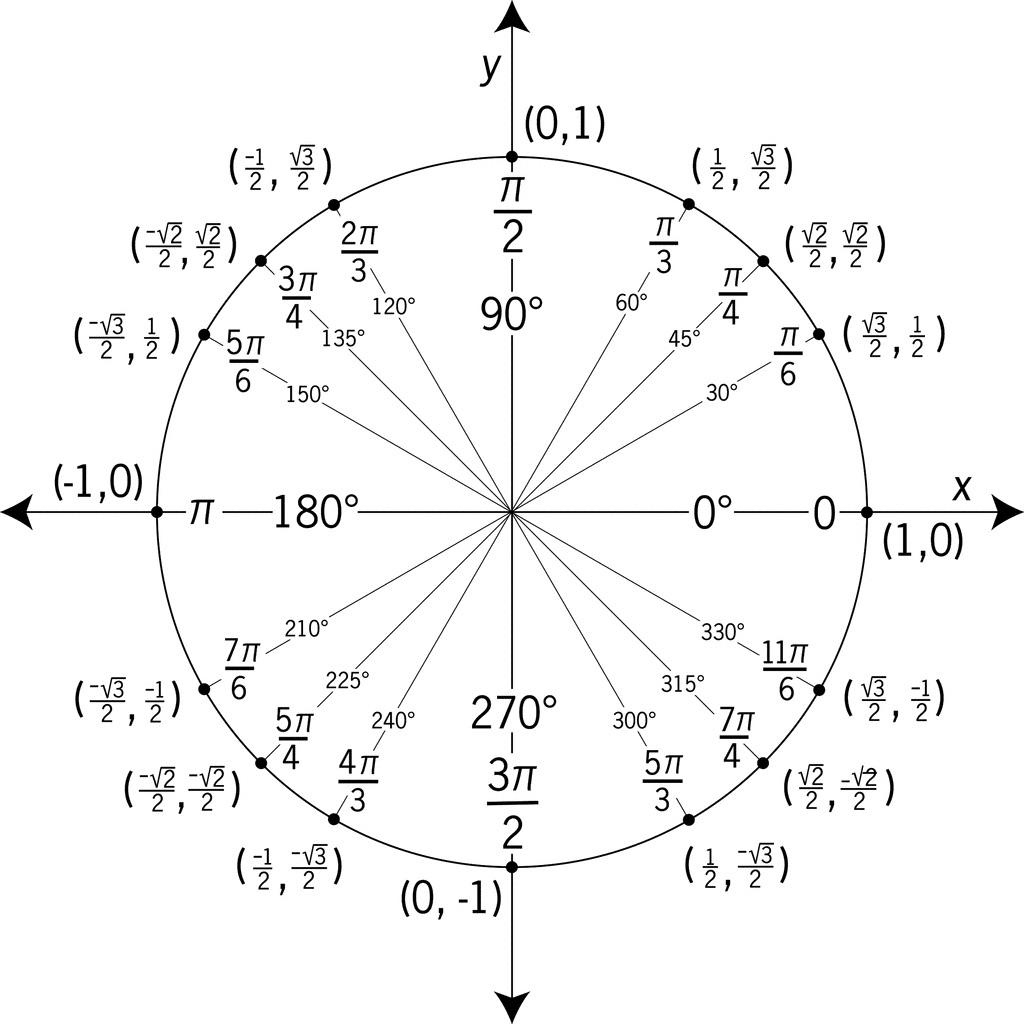
\includegraphics[width=\linewidth,keepaspectratio]{UnitCircle.jpg}\par}
\end{ebox}

\end{multicols}

\vfill
\vspace{2pt}
\noindent
\begin{minipage}[t]{0.19\linewidth}
\shead{purplebg}{purple}{FIELDS}
\begin{ebox}
$\mathbf{E}$ — electric field (V/m)\\
$\mathbf{D}=\varepsilon\mathbf{E}$ — elec.\ flux density (C/m$^2$)\\
$\mathbf{B}$ — mag.\ flux density (T)\\
$\mathbf{H}$ — mag.\ field intensity (A/m)\\
$\rho_v$ — charge density (C/m$^3$)\\
$\rho_{v0}$ — initial charge density\\
$\Phi=\int_S\mathbf{B}\cdot d\mathbf{s}$ — flux (Wb)\\
$\lambda=N\Phi$ — flux linkage (Wb)
\end{ebox}
\end{minipage}\hfill
\begin{minipage}[t]{0.19\linewidth}
\shead{tealbg}{teal}{CURRENTS}
\begin{ebox}
$J_c=\sigma E$ — cond.\ density (A/m$^2$)\\
$J_d=\varepsilon\,\partial E/\partial t$ — disp.\ density\\
$I_c=J_c\cdot A$ — cond.\ current (A)\\
$I_d=J_d\cdot A$ — disp.\ current (A)\\
$R=d/(\sigma A)$ — resistance ($\Omega$)\\
$C=\varepsilon_r\varepsilon_0 A/d$ — capacitance (F)\\
$\tau_r=\varepsilon_r\varepsilon_0/\sigma$ — relax.\ time (s)
\end{ebox}
\end{minipage}\hfill
\begin{minipage}[t]{0.19\linewidth}
\shead{coralbg}{coral}{MATERIALS}
\begin{ebox}
$\mu_0=4\pi\!\times\!10^{-7}$ H/m\\
$\mu_r$ — relative permeability (—)\\
$\mu=\mu_r\mu_0$ — permeability (H/m)\\[2pt]
$\varepsilon_0=8.85\!\times\!10^{-12}$ F/m\\
$\varepsilon_r$ — relative permittivity (—)\\
$\varepsilon=\varepsilon_r\varepsilon_0$ — permittivity (F/m)\\[2pt]
$\sigma$ — conductivity (S/m)
\end{ebox}
\end{minipage}\hfill
\begin{minipage}[t]{0.19\linewidth}
\shead{bluebg}{blue}{CIRCUIT \& WAVE}
\begin{ebox}
$V$ — voltage (V)\\
$R$ — resistance ($\Omega$)\\
$C$ — capacitance (F)\\
$\omega=2\pi f$ — angular freq (rad/s)\\
$k=\omega\sqrt{\mu\varepsilon}$ — wave number (m$^{-1}$)\\
$\lambda=2\pi/k$ — wavelength (m)\\
$c=3\!\times\!10^8$ m/s — speed of light
\end{ebox}
\end{minipage}\hfill
\begin{minipage}[t]{0.19\linewidth}
\shead{pinkbg}{pink}{PHASOR \& GEOMETRY}
\begin{ebox}
$\eta=\sqrt{\mu/\varepsilon}$ — intrinsic imp.\ ($\Omega$)\\
$\eta_0=120\pi\approx377\,\Omega$ (free space)\\
$k/(\omega\mu)=1/\eta$\\
$j$ — imaginary unit ($j^2=-1$)\\
$\tilde{\mathbf{E}}$ — phasor (V/m; drop $e^{j\omega t}$)\\[2pt]
$A$ — area (m$^2$);\quad $d$ — sep.\ (m)\\
$N$ — turns;\quad $r$ — radial dist.\ (m)
\end{ebox}
\end{minipage}

\newpage

%%=============================================================
%% PAGE 2 — HW2 CHEAT SHEET (verbatim)
%%=============================================================
\fontsize{6}{7}\selectfont
\setlength{\abovedisplayskip}{0pt}\setlength{\belowdisplayskip}{0.5pt}
\setlength{\abovedisplayshortskip}{0pt}\setlength{\belowdisplayshortskip}{0pt}
\begin{multicols}{3}

%──────────────────────────────────────
\shead{purplebg}{purple}{PLANE WAVE PARAMETERS (LOSSLESS)}
\begin{ebox}
\eq{Angular frequency}{$\omega$: rad/s;\enspace$f$: Hz}
\[\omega = 2\pi f \qquad f = \frac{\omega}{2\pi}\]

\eq{Phase velocity}{m/s;\enspace nonmagnetic: $\mu_r=1$}
\[u_p = \frac{c}{\sqrt{\varepsilon_r}} \qquad c = 3\times10^8\;\text{m/s}\]

\eq{Wavenumber $k$}{rad/m}
\[k = \frac{\omega}{u_p} = \frac{2\pi}{\lambda} = \frac{\omega\sqrt{\varepsilon_r}}{c}\]

\eq{Wavelength \& impedance}{m \& $\Omega$}
\[\lambda = \frac{u_p}{f} = \frac{2\pi}{k}\;\text{(m)} \qquad \eta = \frac{\eta_0}{\sqrt{\varepsilon_r}}\;(\Omega),\;\eta_0=377\,\Omega\]

\textit{\color{coral}Order: $\omega\!\to\!u_p\!\to\!k\!\to\!\lambda\!\to\!\eta$.\enspace Base: $\mathbf{E}\!=\!E_0\cos(\omega t\pm kx+\phi_0)\hat{e}$.}
\end{ebox}

\vspace{0.3pt}
\shead{purplebg}{purple}{LOSSLESS PLANE WAVE --- $\mathbf{E}$ AND $\mathbf{H}$}
\begin{ebox}
\eq{General $\mathbf{E}$}{}
\[\mathbf{E} = E_0\cos(\omega t - k\,\hat{k}\cdot\mathbf{r} + \phi_0)\,\hat{e}\]
\textit{$\hat{k}$ = direction of travel (unit vector), e.g.\ $+y\Rightarrow\hat{k}=\hat{y}$.}\\
\textit{$k$ = wavenumber (rad/m): how fast phase changes in space; $k=\omega\sqrt{\varepsilon_r}/c=2\pi/\lambda$.}\\
\textit{$\phi_0$ = initial phase constant (rad): shift set by given condition at known $t$, position.}\\
\textit{$\hat{e}$ = polarization direction of $\mathbf{E}$ (unit vector), e.g.\ E along $x\Rightarrow\hat{e}=\hat{x}$.}\\
\textit{$\mathbf{r}=x\hat{x}+y\hat{y}+z\hat{z}$, so $\hat{k}\cdot\mathbf{r}$ picks the axis, e.g.\ $\hat{k}=\hat{y}\Rightarrow\hat{k}\cdot\mathbf{r}=y$.}

\eq{$\mathbf{H}$ from $\mathbf{E}$}{$\hat{k}$, $\hat{E}$, $\hat{H}$ form right-hand set}
\[\mathbf{H} = \frac{1}{\eta}\,(\hat{k}\times\mathbf{E})\]

\eq{Find $\phi_0$}{given $E=E_1$ at $t=0$, position $r_0$}
\[E_0\cos(-kr_0+\phi_0)=E_1\;\Rightarrow\;\phi_0=\cos^{-1}\!\!\left(\tfrac{E_1}{E_0}\right)+kr_0\]
\textit{\color{coral}$\cos^{-1}$ gives $[0,\pi]$; take $\phi_0$ in that range.}
\end{ebox}

\vspace{0.3pt}
\shead{bluebg}{blue}{LOSSLESS vs.\ LOSSY --- E \& H}
\begin{ebox}
{\centering\makebox[0.98\linewidth][c]{{\setlength{\tabcolsep}{2pt}\begin{tabular}{@{}p{0.20\linewidth}|>{\centering\arraybackslash}p{0.35\linewidth}|>{\centering\arraybackslash}p{0.37\linewidth}@{}}
\toprule
& \textbf{Lossless} ($\sigma\!=\!0$) & \textbf{Lossy} ($\sigma\!\ne\!0$)\\
\midrule
\rowcolor{rowB}Impedance & $\eta=\sqrt{\mu/\varepsilon}$ & $\eta_c=|\eta_c|e^{j\theta_\eta}$\\
Prop. & $e^{-jkz}$ & $e^{-\alpha z}e^{-j\beta z}$\\
\rowcolor{rowB}$\mathbf{E}(t)$ & \multicolumn{2}{c}{$\operatorname{Re}\{\tilde{\mathbf{E}}\,e^{j\omega t}\}$ \textit{(same)}}\\
$\mathbf{H}(t)$ & \multicolumn{2}{c}{$\operatorname{Re}\{\tilde{\mathbf{H}}\,e^{j\omega t}\}$ \textit{(same)}}\\
\rowcolor{rowB}$\tilde{\mathbf{H}}$ from $\tilde{\mathbf{E}}$ & $\tfrac{1}{\eta}(\hat{k}\times\tilde{\mathbf{E}})$ & $\tfrac{1}{\eta_c}(\hat{k}\times\tilde{\mathbf{E}})$\\
$\tilde{\mathbf{E}}$ from $\tilde{\mathbf{H}}$ & $-\eta(\hat{k}\times\tilde{\mathbf{H}})$ & $-\eta_c(\hat{k}\times\tilde{\mathbf{H}})$\\
\rowcolor{rowB}Phase & in phase & H lags E by $\theta_\eta$\\
\midrule
\multicolumn{3}{l}{\textit{Lossless shortcuts (wave in $+z$, $\mathbf{E}$ along $\hat{e}$):}}\\
\rowcolor{rowB}$\mathbf{E}(z,t)$ & \multicolumn{2}{l}{$E_0\cos(\omega t-kz+\phi)\,\hat{e}$}\\
$\mathbf{H}(z,t)$ & \multicolumn{2}{l}{$\tfrac{E_0}{\eta}\cos(\omega t-kz+\phi)\,(\hat{k}\times\hat{e})$}\\
\rowcolor{rowB}$\mathbf{H}(t)$ direct & \multicolumn{2}{l}{$\tfrac{1}{\eta}(\hat{k}\times\mathbf{E}(t))$}\\
$\mathbf{E}(t)$ direct & \multicolumn{2}{l}{$-\eta(\hat{k}\times\mathbf{H}(t))$}\\
\bottomrule
\end{tabular}}}\par}
\end{ebox}

\vspace{0.3pt}
\shead{purplebg}{purple}{DIRECTION OF PROPAGATION}
\begin{ebox}
\makebox[0.92\linewidth][c]{\begin{tabular}{@{}ll@{\quad}ll@{}}
\toprule
Arg.\ contains & $\hat{k}$ & Arg.\ contains & $\hat{k}$\\
\midrule
\rowcolor{rowB}$\omega t-kz$ & $+\hat{z}$ & $\omega t+kz$ & $-\hat{z}$\\
$\omega t-ky$ & $+\hat{y}$ & $\omega t+ky$ & $-\hat{y}$\\
\rowcolor{rowB}$\omega t-kx$ & $+\hat{x}$ & $\omega t+kx$ & $-\hat{x}$\\
\bottomrule
\end{tabular}}\\[1pt]
\textit{Minus before $k$-axis $\Rightarrow$ $+$ direction. Plus $\Rightarrow$ $-$ direction.}
\end{ebox}

\vspace{0.3pt}
\shead{tealbg}{teal}{$\hat{k}\times\hat{E}$ --- FIND $\hat{H}$ DIRECTION}
\begin{ebox}
\makebox[0.98\linewidth][c]{\begin{tabular}{@{}lll|lll@{}}
\toprule
$\hat{k}$ & $\hat{E}$ & $\hat{H}$ & $\hat{k}$ & $\hat{E}$ & $\hat{H}$\\
\midrule
\rowcolor{rowB}$+\hat{z}$ & $\hat{x}$ & $+\hat{y}$ & $+\hat{z}$ & $\hat{y}$ & $-\hat{x}$\\
$-\hat{z}$ & $\hat{x}$ & $-\hat{y}$ & $-\hat{z}$ & $\hat{y}$ & $+\hat{x}$\\
\rowcolor{rowB}$+\hat{y}$ & $\hat{x}$ & $-\hat{z}$ & $+\hat{y}$ & $\hat{z}$ & $+\hat{x}$\\
$-\hat{y}$ & $\hat{x}$ & $+\hat{z}$ & $-\hat{y}$ & $\hat{z}$ & $-\hat{x}$\\
\rowcolor{rowB}$+\hat{x}$ & $\hat{y}$ & $+\hat{z}$ & $+\hat{x}$ & $\hat{z}$ & $-\hat{y}$\\
$-\hat{x}$ & $\hat{y}$ & $-\hat{z}$ & $-\hat{x}$ & $\hat{z}$ & $+\hat{y}$\\
\bottomrule
\end{tabular}}\\[1pt]
\textit{Neg.\ $\hat{E}$: flip $\hat{H}$ sign.\enspace$\hat{k}\!\times\!\hat{k}\!=\!\mathbf{0}$;\enspace any $\hat{a}\!\times\!\hat{a}\!=\!\mathbf{0}$.}\\
\textit{Cyclic: $\hat{x}\!\times\!\hat{y}\!=\!\hat{z}$, $\hat{y}\!\times\!\hat{z}\!=\!\hat{x}$, $\hat{z}\!\times\!\hat{x}\!=\!\hat{y}$. Reverse $\Rightarrow$ flip sign.}
\end{ebox}

\vspace{0.3pt}
\shead{graybg}{gray}{TRIG PHASE SHIFTS \textnormal{\textit{($\theta\!\equiv\!\omega t\!-\!kz$)}}}
\begin{ebox}
{\centering\makebox[0.98\linewidth][c]{{\setlength{\tabcolsep}{2pt}\begin{tabular}{@{}p{0.25\linewidth}p{0.18\linewidth}p{0.25\linewidth}p{0.18\linewidth}@{}}
\toprule
Input & Result & Input & Result\\
\midrule
\rowcolor{rowB}$\sin(\theta{+}\pi/2)$ & $\cos\theta$ & $\cos(\theta{+}\pi/2)$ & $-\sin\theta$\\
$\sin(\theta{-}\pi/2)$ & $-\cos\theta$ & $\cos(\theta{-}\pi/2)$ & $\sin\theta$\\
\rowcolor{rowB}$\sin(\theta{+}\pi)$ & $-\sin\theta$ & $\cos(\theta{+}\pi)$ & $-\cos\theta$\\
$\sin(\theta{-}\pi)$ & $-\sin\theta$ & $\cos(\theta{-}\pi)$ & $-\cos\theta$\\
\bottomrule
\end{tabular}}}\par}
\end{ebox}

\columnbreak

%──────────────────────────────────────
\shead{tealbg}{teal}{POLARIZATION --- GENERAL WAVE}
\begin{ebox}
{\centering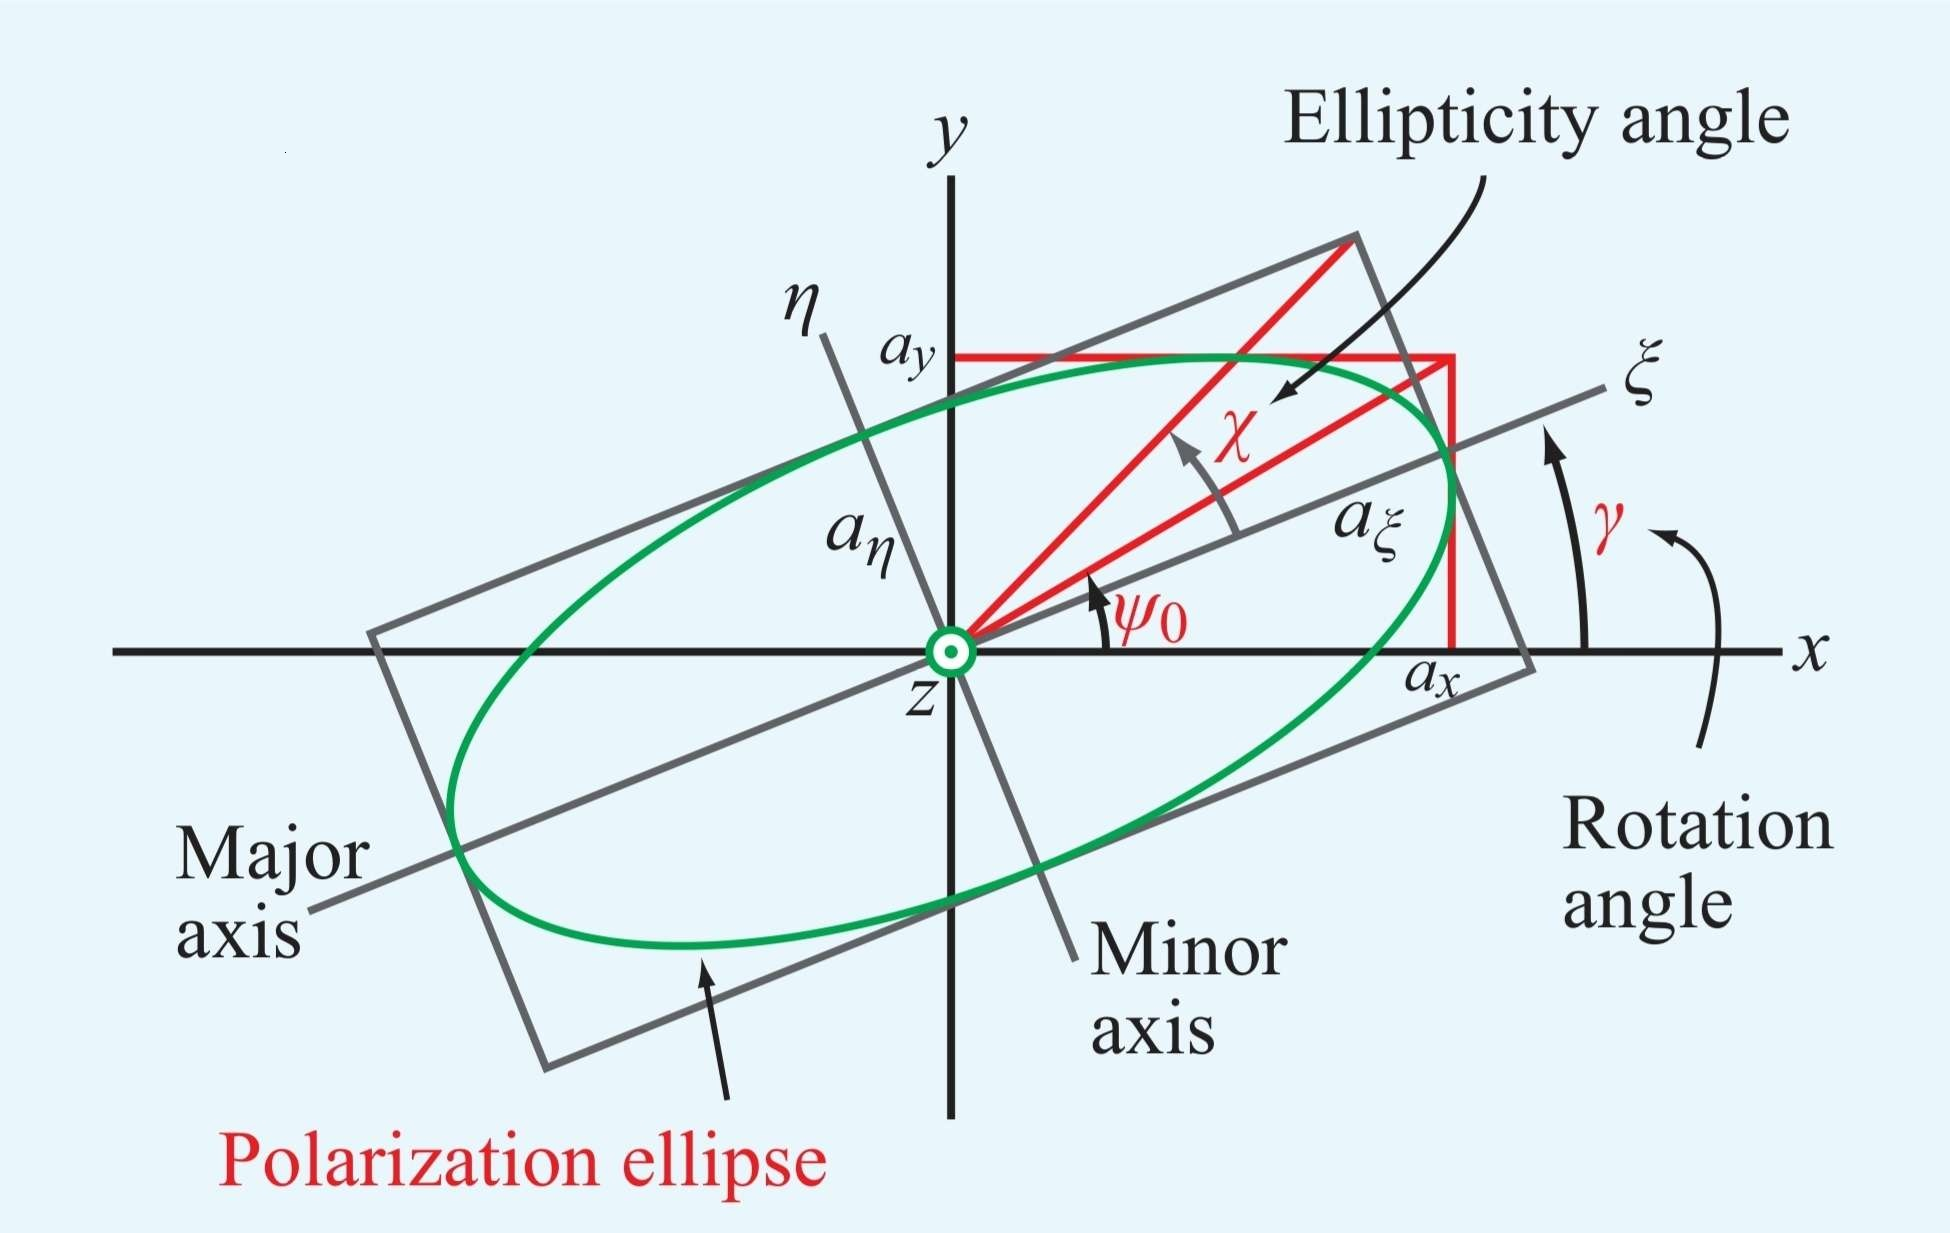
\includegraphics[width=\linewidth,keepaspectratio]{pol_ellipse.jpg}\par}
\vspace{-8pt}
\[\mathbf{E}=a_x\cos(\omega t\!-\!kz)\hat{x}+a_y\cos(\omega t\!-\!kz+\delta)\hat{y}\]
\textit{$a_x,a_y$: bounding box half-widths (V/m);\enspace$\delta$: phase diff (rad)}\\
\textit{\color{gray}$\delta=0$: $\mathbf{E}=(a_x\hat{x}+a_y\hat{y})\cos(\omega t\!-\!kz)$\textbf{ (linear)}}\\
\textit{\color{gray}$\delta=\pi$: $\mathbf{E}=(a_x\hat{x}-a_y\hat{y})\cos(\omega t\!-\!kz)$\textbf{ (linear)}}\\
\eq{Auxiliary angle}{$\psi_0=\arctan(a_y/a_x)\in(0,\pi/2)$}\\
\eq{Rotation angle $\gamma$ (major axis from $\hat{x}$)}{$\gamma\in[0,\pi)$}
\[\tan(2\gamma)=\tan(2\psi_0)\cos\delta\]
\textit{\color{coral}If sign$(\gamma)\!\neq\!$sign$(\delta)$: $\gamma\leftarrow\gamma\pm\tfrac{\pi}{2}$.}\\
\eq{Ellipticity angle $\chi$}{$\chi\in[-\pi/4,\pi/4]$}
\[\sin(2\chi)=\sin(2\psi_0)\sin\delta\]
\eq{Axial ratio $R=1/\tan|\chi|$}{major axis $=R\times$ minor;\enspace$R\geq1$}
\end{ebox}

\vspace{0.3pt}
\shead{tealbg}{teal}{$\chi$ SHAPE \& HANDEDNESS}
\begin{ebox}
\textit{$\chi$ describes the shape of the ellipse and rotation direction.}\\[1pt]
{\centering\makebox[0.98\linewidth][c]{{\setlength{\tabcolsep}{2pt}\begin{tabular}{@{}p{0.30\linewidth}p{0.33\linewidth}p{0.30\linewidth}@{}}
\toprule
$\chi$ (rad) & Polarization Type & Handedness\\
\midrule
\rowcolor{rowB}$0$ & Linear & None\\
$(0,\,\pi/4)$ & RHEP & RH (CCW)\\
\rowcolor{rowB}$\pi/4$ & RHC & RH (CCW)\\
$-\pi/4$ & LHC & LH (CW)\\
\rowcolor{rowB}$(-\pi/4,\,0)$ & LHEP & LH (CW)\\
\bottomrule
\end{tabular}}}\par}
\end{ebox}

\vspace{0.3pt}
\shead{tealbg}{teal}{QUADRANT RULE FOR $\tan(2\gamma)$}
\begin{ebox}
$N=\sin(2\psi_0)\cos\delta$,\quad $D=\cos(2\psi_0)$:\\[1pt]
{\centering\makebox[0.98\linewidth][c]{\begin{tabular}{@{}ccll@{}}
\toprule
$N$ & $D$ & $2\gamma$ (deg) & $2\gamma$ (rad)\\
\midrule
\rowcolor{rowB}$+$ & $+$ & $\arctan(N/D)$ & $\arctan(N/D)$\\
$+$ & $-$ & $180^\circ-\arctan|N/D|$ & $\pi-\arctan|N/D|$\\
\rowcolor{rowB}$-$ & $-$ & $180^\circ+\arctan|N/D|$ & $\pi+\arctan|N/D|$\\
$-$ & $+$ & $360^\circ-\arctan|N/D|$ & $2\pi-\arctan|N/D|$\\
\bottomrule
\end{tabular}}\par}\vspace{1pt}
\textit{$\gamma=(2\gamma)/2$.\quad $D=0\Rightarrow2\gamma=\tfrac{\pi}{2}\Rightarrow\gamma=\tfrac{\pi}{4}$.}\\[0.5pt]
\textit{Convert: $\theta_\text{rad}=\theta_\circ\times\tfrac{\pi}{180}$;\enspace$\theta_\circ=\theta_\text{rad}\times\tfrac{180}{\pi}$.}
\end{ebox}

\vspace{0.3pt}
\shead{pinkbg}{pink}{PHASOR $\leftrightarrow$ TIME DOMAIN}
\begin{ebox}
{\centering\makebox[0.98\linewidth][c]{{\setlength{\tabcolsep}{2pt}\begin{tabular}{@{}p{0.17\linewidth}p{0.41\linewidth}p{0.35\linewidth}@{}}
\toprule
Phasor coeff & $\operatorname{Re}\{(\cdot)\,e^{j\omega t}e^{-j\beta z}\}$ & Result\\
\midrule
\rowcolor{rowB}$A$ & $\operatorname{Re}\{Ae^{j(\omega t-\beta z)}\}$ & $A\cos(\omega t\!-\!\beta z)$\\
$-jA$ & $\operatorname{Re}\{Ae^{j(\omega t-\beta z-\pi/2)}\}$ & $A\sin(\omega t\!-\!\beta z)$\\
\rowcolor{rowB}$+jA$ & $\operatorname{Re}\{Ae^{j(\omega t-\beta z+\pi/2)}\}$ & $-A\sin(\omega t\!-\!\beta z)$\\
$-A$ & $\operatorname{Re}\{Ae^{j(\omega t-\beta z\pm\pi)}\}$ & $-A\cos(\omega t\!-\!\beta z)$\\
\rowcolor{rowB}$Ae^{j\phi}$ & $\operatorname{Re}\{Ae^{j(\omega t-\beta z+\phi)}\}$ & $A\cos(\omega t\!-\!\beta z\!+\!\phi)$\\
$A+jB$ & $\operatorname{Re}\{|Z|e^{j(\omega t-\beta z+\theta)}\}$ & $|Z|\cos(\omega t\!-\!\beta z\!+\!\theta)$\\
\bottomrule
\end{tabular}}}\par}\vspace{1pt}
$|Z|=\sqrt{A^2+B^2}$,\enspace$\theta=\arctan(B/A)$ (check quadrant)
\end{ebox}

\vspace{0.3pt}
\shead{amberbg}{amber}{CIRCULAR POLARIZATION --- TIME DOMAIN}
\begin{ebox}
\textit{$a_x=a_y=a$, wave in $+\hat{z}$}\\
\eq{RHC}{$\delta=-\pi/2$;\enspace$\tilde{\mathbf{E}}=a(\hat{x}-j\hat{y})e^{-jkz}$}
\[\mathbf{E}(z,t)=a\bigl[\cos(\omega t\!-\!kz)\,\hat{x}+\sin(\omega t\!-\!kz)\,\hat{y}\bigr]\]
\eq{LHC}{$\delta=+\pi/2$;\enspace$\tilde{\mathbf{E}}=a(\hat{x}+j\hat{y})e^{-jkz}$}
\[\mathbf{E}(z,t)=a\bigl[\cos(\omega t\!-\!kz)\,\hat{x}-\sin(\omega t\!-\!kz)\,\hat{y}\bigr]\]
\end{ebox}

\vspace{2pt}
\shead{amberbg}{amber}{RETARDED POTENTIALS}
\begin{ebox}
\[\mathbf{B}=\nabla\times\mathbf{A} \qquad \mathbf{E}=-\nabla V-\frac{\partial\mathbf{A}}{\partial t}\]
\[V(\mathbf{R},t)=\frac{1}{4\pi\varepsilon}\int_{V'}\frac{\rho_v\!\left(\mathbf{R}_i,\,t-R'/u_p\right)}{R'}\,dV' \quad\text{(V)}\]
\[A(\mathbf{R},t)=\frac{\mu}{4\pi}\int_{V'}\frac{\mathbf{J}\!\left(\mathbf{R}_i,\,t-R'/u_p\right)}{R'}\,dV' \quad\text{(Wb/m)}\]
$R'\!=\!|\mathbf{R}\!-\!\mathbf{R}_i|$ (m) src$\to$obs dist;\quad $t\!-\!R'/u_p$: retarded time\\
$u_p\!\approx\!c$;\quad $\rho_v$(C/m$^3$);\quad $\mathbf{J}$(A/m$^2$);\quad $V$(V);\quad $\mathbf{A}$(Wb/m)
\end{ebox}

\columnbreak

%──────────────────────────────────────
\shead{coralbg}{coral}{LOSSY MEDIA --- CLASSIFICATION}
\begin{ebox}
\eq{Loss tangent}{}
\[\frac{\varepsilon''}{\varepsilon'}=\frac{\sigma}{\omega\varepsilon_r\varepsilon_0}\]

{\centering\makebox[0.98\linewidth][c]{{\setlength{\tabcolsep}{2pt}\begin{tabular}{@{}p{0.25\linewidth}p{0.36\linewidth}p{0.3\linewidth}@{}}
\toprule
$\varepsilon''/\varepsilon'$ & Type & Use\\
\midrule
\rowcolor{rowB}$>100$ & Good conductor & GC approx\\
$0.01$ to $100$ & Quasi-conductor & Exact eqs\\
\rowcolor{rowB}$<0.01$ & Low-loss dielectric & LD approx\\
\bottomrule
\end{tabular}}}\par}
\textit{$\varepsilon'=\varepsilon_r\varepsilon_0$;\;$\varepsilon''=\sigma/\omega$;\;nonmag.: $\mu=\mu_0$;\;free space: $\varepsilon_r=\mu_r=1$.}
\end{ebox}

\vspace{0.3pt}
\shead{coralbg}{coral}{ANY MEDIUM --- EXACT ($X=\sqrt{1+(\varepsilon''/\varepsilon')^2}$)}
\begin{ebox}
\[\alpha=\omega\sqrt{\tfrac{\mu\varepsilon'}{2}}\sqrt{X\!-\!1}\,\text{Np/m},\enspace\beta=\omega\sqrt{\tfrac{\mu\varepsilon'}{2}}\sqrt{X\!+\!1}\,\text{rad/m}\]
\[\lambda=\frac{2\pi}{\beta}=\frac{u_p}{f}\;\text{(m)},\quad u_p=\frac{\omega}{\beta}\;\text{(m/s)}\]
\[\eta_c=\frac{\eta}{X^{1/2}}e^{j\theta_\eta}\;(\Omega),\quad\theta_\eta=\tfrac{1}{2}\arctan\!\tfrac{\sigma}{\omega\varepsilon'}\;\text{(rad)}\]
\textit{Rect: $\eta_c=|\eta_c|\cos\theta_\eta+j|\eta_c|\sin\theta_\eta$,\enspace$|\eta_c|=\eta/X^{1/2}$}\\
\textit{$\eta=\eta_0/\sqrt{\varepsilon_r}$;\enspace$\varepsilon'=\varepsilon_r\varepsilon_0$.}\\
\textit{Given $\tilde{\mathbf{H}}\!\propto\!e^{-\alpha y}e^{-j\beta y}$: $\gamma\!=\!\alpha\!+\!j\beta$;\enspace$\eta_c\!=\!j\omega\mu_0/\gamma\!=\!\omega\mu_0(\beta\!+\!j\alpha)/(\alpha^2\!+\!\beta^2)$}
\end{ebox}

\vspace{0.3pt}
\shead{coralbg}{coral}{SKIN DEPTH $\delta_s$ (m) --- ANY LOSSY MEDIUM}
\begin{ebox}
\eq{General: $\delta_s=1/\alpha$}{$|E(z)|=E_0e^{-z/\delta_s}$;\enspace lossless: $\alpha=0\Rightarrow$ no decay}\\
\eq{Low-loss ($\varepsilon''/\varepsilon'\ll1$)}{$\delta_s\approx2/(\sigma\eta)$}\\
\eq{Good conductor ($\varepsilon''/\varepsilon'\gg1$)}{$\delta_s\approx1/\sqrt{\pi f\mu\sigma}$}
\end{ebox}

\vspace{0.3pt}
\shead{coralbg}{coral}{LOW-LOSS MEDIUM ($\varepsilon''/\varepsilon'\ll 1$)}
\begin{ebox}
\[\alpha\approx\tfrac{\sigma}{2}\sqrt{\tfrac{\mu}{\varepsilon'}}=\tfrac{\sigma\eta}{2}\;\text{(Np/m)}\]
\[\beta\approx\omega\sqrt{\mu\varepsilon'}=\tfrac{\omega\sqrt{\varepsilon_r}}{c}\;\text{(rad/m)},\quad u_p\approx\tfrac{c}{\sqrt{\varepsilon_r}}\;\text{(m/s)}\]
\[\eta_c\approx\sqrt{\tfrac{\mu}{\varepsilon'}}=\eta\;(\Omega,\;\angle\approx0)\]
\end{ebox}

\vspace{0.3pt}
\shead{coralbg}{coral}{GOOD CONDUCTOR ($\varepsilon''/\varepsilon'\gg 1$)}
\begin{ebox}
\[\alpha\approx\beta\approx\sqrt{\pi f\mu\sigma}\quad\text{(Np/m, rad/m)}\]
\[u_p\approx\sqrt{4\pi f/\mu\sigma}\;\text{(m/s)},\quad\lambda\approx u_p/f\;\text{(m)}\]
\[\eta_c\approx(1+j)\sqrt{\tfrac{\pi f\mu}{\sigma}}\approx(1+j)\tfrac{\alpha}{\sigma}\quad(\Omega)\]
\end{ebox}

\vspace{0.3pt}
\vspace{0.3pt}
\shead{coralbg}{coral}{SURFACE RESISTANCE (GOOD CONDUCTOR)}
\begin{ebox}
{\centering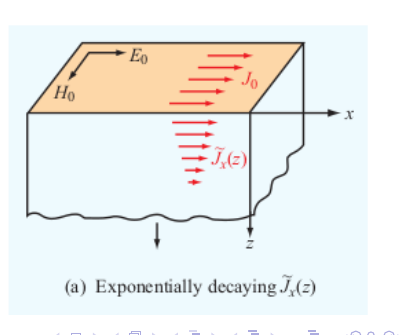
\includegraphics[width=0.55\linewidth,keepaspectratio]{conductor_3d.png}\par}
$J_0=\sigma E_0$ — current density at surface (z=0)\\
$\tilde{\mathbf{J}}(z)=J_0 e^{-(1+j)z/\delta_s}\hat{x}$ — decays with depth\\[1pt]
$R_s=\sqrt{\pi f\mu/\sigma}=1/(\sigma\delta_s)\;(\Omega)$\\
$Z_s=(1+j)R_s$ — surface impedance\\
$R_\text{AC}=R_s\,\ell/w$ — AC resistance of slab
\end{ebox}

\vspace{0.3pt}
\shead{greenbg}{green}{AVERAGE POWER DENSITY (POYNTING)}
\begin{ebox}
\eq{General}{W/m$^2$}
\[\mathbf{S}_\text{av}=\tfrac{1}{2}\operatorname{Re}\{\tilde{\mathbf{E}}\times\tilde{\mathbf{H}}^*\}\]

\eq{Lossless shortcut}{$|E_0|^2=a_x^2+a_y^2+a_z^2$}
\[\mathbf{S}_\text{av}=\frac{|E_0|^2}{2\eta}\,\hat{k}\]

\eq{Lossy medium}{$\eta_c=|\eta_c|e^{j\theta_\eta}$; wave in $+\hat{z}$}
\[\mathbf{S}_\text{av}=\frac{|\tilde{\mathbf{E}}(0)|^2}{2|\eta_c|}e^{-2\alpha z}\cos\theta_\eta\;\hat{z}\]

\textit{Direction = $\hat{k}$. If wave goes in $-\hat{x}$, then $\mathbf{S}_\text{av}$ is a negative $x$-component.}
\end{ebox}

\vspace{0.3pt}
\shead{greenbg}{green}{DECIBELS \& ATTENUATION}
\begin{ebox}
$G=10\log(P_1/P_2)=20\log(|E_1|/|E_2|)$ (dB)\\
$A=-8.69\,\alpha\,z$ (dB);\enspace$\alpha\,\text{(dB/m)}\equiv8.69\,\alpha\,\text{(Np/m)}$
\end{ebox}

\end{multicols}

\vfill
\noindent
\begin{minipage}[t]{0.19\linewidth}
\shead{purplebg}{purple}{WAVE PARAMS}
\begin{ebox}
$\omega=2\pi f$ --- ang.\ freq (rad/s)\\
$k=\omega\sqrt{\varepsilon_r}/c$ --- wavenumber (rad/m)\\
$\lambda=2\pi/k$ --- wavelength (m)\\
$u_p=c/\sqrt{\varepsilon_r}$ --- phase vel.\ (m/s)\\
$\eta=\eta_0/\sqrt{\varepsilon_r}$ --- impedance ($\Omega$)\\
$c=3\times10^8$ m/s\\
\textbf{$\eta_0=377\,\Omega$} (free space)
\end{ebox}
\end{minipage}\hfill
\begin{minipage}[t]{0.19\linewidth}
\shead{purplebg}{purple}{LOSSLESS MEDIA}
\begin{ebox}
$\sigma=0$ (vacuum, air, ideal dielectric)\\
$\varepsilon''=\sigma/\omega=0\;\Rightarrow\;\varepsilon=\varepsilon'$ (real)\\
$\alpha=0$;\enspace no attenuation\\
$\eta=\eta_0/\sqrt{\varepsilon_r}$ real ($\Omega$)\\
$\eta_0=377\,\Omega$ (free space)\\
$\mathbf{E}$ and $\mathbf{H}$ in phase ($\theta_\eta=0$)
\end{ebox}
\end{minipage}\hfill
\begin{minipage}[t]{0.19\linewidth}
\shead{coralbg}{coral}{LOSSY MEDIA}
\begin{ebox}
$\alpha$ --- atten.\ const (Np/m)\\
$\beta$ --- phase const (rad/m)\\
$\gamma=\alpha+j\beta$ --- prop.\ const (m$^{-1}$)\\
$\eta_c$ --- complex impedance ($\Omega$)\\
$\varepsilon'=\varepsilon_r\varepsilon_0$;\;$\varepsilon''=\sigma/\omega$ (F/m)\\
$\mu_r$ --- rel.\ permeability ($\mu_r=1$: nonmagnetic)\\
$\mu=\mu_r\mu_0$;\;$\mu_0=4\pi\times10^{-7}$ H/m\\
$\delta_s=1/\alpha$ --- skin depth (m)
\end{ebox}
\end{minipage}\hfill
\begin{minipage}[t]{0.19\linewidth}
\shead{amberbg}{amber}{CIRCULAR WAVES}
\begin{ebox}
$\tilde{\mathbf{E}}_R=a_R(\hat{x}+e^{-j\pi/2}\hat{y})e^{-jkz}=a_R(\hat{x}-j\hat{y})e^{-jkz}$\\
$\tilde{\mathbf{E}}_L=a_L(\hat{x}+e^{+j\pi/2}\hat{y})e^{-jkz}=a_L(\hat{x}+j\hat{y})e^{-jkz}$\\
$a_R,a_L,a_x$ in V/m;\;$k$ in rad/m\\
Linear: $a_R=a_L=a_x/2$\\
$-j=e^{-j\pi/2}$: cos$\to$sin\\
$+j=e^{+j\pi/2}$: cos$\to{-}$sin
\end{ebox}
\end{minipage}\hfill
\begin{minipage}[t]{0.19\linewidth}
\shead{amberbg}{amber}{DECIBEL VARIABLES}
\begin{ebox}
$G$: power gain (dB)\\
$P_1,P_2$: power (W)\\
$|E_1|,|E_2|$: field (V/m)\\
$A$: atten.\ over $z$ (dB)\\
$\alpha$: atten.\ const (Np/m)\\
$z$: dist (m)\\
$P\!\propto\!E^2\!\Rightarrow$ 20 log not 10\\
Np/m $\times$ 8.69 = dB/m
\end{ebox}
\end{minipage}

\end{document}
